\documentclass[__main__.tex]{subfiles}

\begin{document}

\qtitle{К}{15}
Рассмотрите задачу об одномерном потенциальном барьере бесконечной ширины для случая, когда энергия микрообъекта превышает высоту потенциального порога, найдите коэффициенты отражения и прохождения.\\

\begin{wrapfigure}{L}{.3\linewidth}
    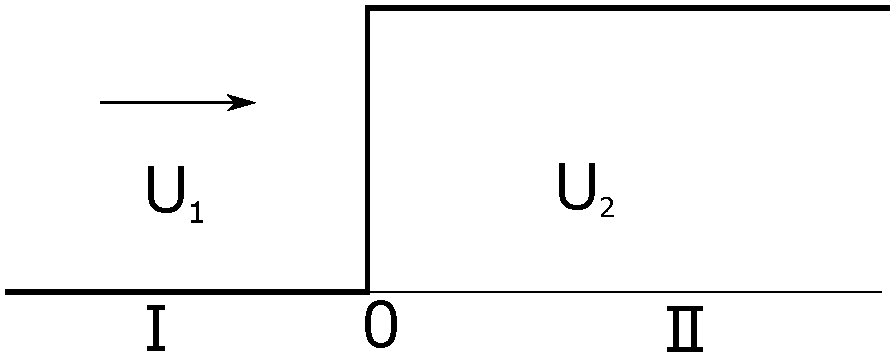
\includegraphics[width=1\linewidth]{k-15}
    \caption{}
    \llabel{k15:1}
\end{wrapfigure}
Рассмотрим одномерный потенциальный барьер, когда потенциальная функция $U$ зависит только от одной координаты $x$. Потенциальным барьером такого типа называется ограниченная параллельными плоскостями область пространства, в которой потенциальная функция $U(x)$ больше, чем в примыкающих областях.\\
Начнём с простейшего идеализированного случая прямоугольного потенциального барьера, когда одна из его стенок удалена в бесконечность. Такой барьер может быть назван ступенчатым, так как \textbf{потенциальная функция $U(x)$ в этом случае представляется ступенчатой линией (см. Рис. \lref{k15:1})}:
\begin{gather}
    U(x) =
    \begin{cases}
        U_1 = const\text{ в области I, где }x<0  \\
        U_2 = const\text{ в области II, где }x>0 \\
    \end{cases},
\end{gather}
причём $U_2>U_1$. На границу барьера слева с постоянной скоростью налетает частица или поток частиц. С классической точки зрения ведёт себя по-разному в зависимости от того, будет ли её полная энергия $\mathbb{\varepsilon}$ больше или меньше $U_2$. В первом случае, когда $\mathcal{\varepsilon}>U_2$, частица, достигнув граница барьера, будет продолжать движение в прежнем направлении, но с меньшей кинетической энергией. Во втором случае, когда $\varepsilon < U_2$, частица вообще не может проникнуть через границу барьера. Она отразится от него и начнёт движение в обратном направлении с той же кинетической энергией.\\
Совсем иное решение задачи даёт квантовая механика. Здесь \textbf{движение частицы}, хотя и символически, \textbf{связано с распространением волны}. Основное уравнение квантовой механики - \textbf{уравнение Шрёдингера - описывает} (и притом детерменически) \textbf{распространение} именно \textbf{волн, а не движение частиц}. Переход же от поведения волн к движению частиц устанавливается вероятностными законами. Поэтому поставленная нами задача должна быть переформулирована, а затем решена для волн на основе уравнения Шрёдингера. Последнее мы будем записывать в виде
\begin{gather}
    \frac{d^2\psi}{dx^2} + k^2\psi = 0,
\end{gather}
где
\begin{gather}
    k^2 = \frac{2m}{\hbar^2}(\mathcal{\varepsilon} - U),
\end{gather}
причём $U$ имеет разные, но постоянные значения $U_1$ и $U_2$ по разные стороны границы барьера. Соответствующие им значения $k$ обозначаются через $k_1$ и $k_2$.\\
Вместо потока частиц теперь надо предположить, что в области $I$ к границе барьера распространяется плоская монохроматическая волна $\psi_1 = e^{i(k_1x-\omega t)}$.\\
Чтобы удовлетворялись граничные условия для $\psi$ и $d\psi/dx$ на границе барьера, в области $I$ должна существовать отражённая волна
\begin{gather*}
    \psi_1' = re^{-i(k_1x+\omega t)},
\end{gather*}
в области $II$ - прошедшая волна    \begin{gather*}
    \psi_2 = de^{i(k_2x - \omega t)}.
\end{gather*}
Амплитуда падающей волны принята равной единице, что, очевидно, не нарушает общности получаемых ниже результатов. \textbf{Постоянные $r$ и $d$ называются амплитудными коэффициентами отражения и пропускания волн}. Для их определения заметим, что функция $\psi$ и её производная по $x$ на границе барьера должны быть непрерывны. Это значит, что при $x = 0$ должны выполняться соотношения
\begin{gather*}
    (\psi_1 + \psi_1') = \psi_2, \hspace{3mm} \frac{d}{dx}(\psi_1 + \psi_1') = \frac{d\psi_2}{dx},
\end{gather*}
или
\begin{gather*}
    l + r = d, \hspace{3mm} k_1 - k_1r = k_2d.\\
    r = \frac{k_1-k_2}{k_1 + k_2}, \hspace{3mm} d = \frac{2k_1}{k_1 + k_2}.
\end{gather*}

\end{document}